\documentclass[12pt,twosides]{article}
\usepackage{jmlda, amsmath, amssymb}
\usepackage{hyperref}
\usepackage{graphicx}
%\NOREVIEWERNOTES

\usepackage{wrapfig}
\usepackage{subfloat}
\usepackage{caption}

\graphicspath{{../pics/}}
%\epstopdfDeclareGraphicsRule{.pdf}{png}{.png}{convert #1 \OutputFile}
%\DeclareGraphicsExtensions{.png,.pdf}

\title
[Графовые сверточные сети для оценки качества структуры белка]
{Оценка качества прогнозирования структуры белка с использованием графовых сверточных нейронных сетей.}
\author
[Северилов~П.А.] 
{Северилов~П.А.$^1$} 
% [] список авторов, выводимый в заголовок; не нужен, если он не отличается от основного
\thanks
{Научный руководитель:  В.В. Стрижов
}
\email
{severilov.pa@phystech.edu}
\organization
{$^1$Московский физико-технический институт (МФТИ)}
\abstract
{Решается задача оценки качества прогнозирования белковых структур. Спектральная теория графов определяет свертку в нейронных сетях при работе с данными в виде графов. Описание белковых структур представлено в виде графов. В работе рассматриваются результаты применения графовых сверточных нейронных сетей к задаче оценивания предсказания белковой структуры. 
	
	\bigskip
	\textbf{Ключевые слова}: \emph {белковые структуры, графы, графовые нейронные сети, спектральные свертки}.}


\begin{document}
	\maketitle
	%\linenumbers
	
	\section{Введение}
	
	Белки являются наиболее универсальными макромолекулами в живых системах и выполняют важнейшие функции практически во всех биологических процессах\cite{berg2002biochemistry}. (?Понимание белковых структур и выполняемых задач помогают контроллировать биологические процессы.?)
	%Белки спонтанным образом принимают форму в различных средах [?] -- 
	Форма белковой структуры определяет (дикутет) её функционал\cite{berg2002biochemistry}. Но из имеющихся последовательностей аминокислот в белке трудно определить, в какую форму сворачивается структура. Идентификация структуры занимает большое количество времени и ресурсов, к тому же, не всегда возможна. 
	
	Каждые два года проводятся соревнования Critical Assessment of protein Structure Prediction (\href{http://predictioncenter.org/}{CASP}) по решению задачи предсказания структуры. 	Вычислительные методы, которые решают её состоят из двух этапов: генерация конформаций белка из их аминокислотных последовательностей и оценивание качества предсказания. В данной работе рассматривается только второй этап.
	
	Белковая структура состоит из одной или нескольких цепочек более мелких молекул -- аминокислотных остатков. Последовательность остатков S = $\{a_i\}_{i=1}^N$ представляет его первичную структуру, где $a_i$ является одним из 22 типов аминокислот. Взаимодействия между соседними остатками и окружающей средой определяют, как цепочка будет сворачиваться в сложные структуры, которые представляют вторичную структуру и третичную структуру белка.
	
	Поэтому для задач с участием белковых структур модель должна учитывать как пространственную информацию об атомах, т.е. третичную структуру, так и признаки в виде последовательностей, т.е. первичную структуру белка.  В работах \cite{HurtadoQA, AngularQA} для моделирования белков используются LSTM или 1D-CNN, которые представляют белки в виде последовательности с пространственными признаками.  В работах \cite{3DCNN, 10.1093/bioinformatics/btz122} моделируется пространственная структура белков с использованием 3D-CNN, но не учитывается структура последовательностей. На основе графов моделируются как последовательности, так и геометрические структуры белков. В работе \cite{Baldassarre2019GraphQAPM} графовые нейронные сети на основе алгоритма, описанного в \cite{Battaglia2018RelationalIB}, показывают результаты, превосходящие остальные современные методы. 
	%Кроме того, графы инвариантны к поворотам и сдвигам, может получать на вход белки разных размеров. 
	
	
	%До недавнего времени лучшими методами предсказания стурктуры считались[?...?] объединение подходов, основанных на функциях, предназначенных для узкого класса белков. Методы глубинного обучения превзошли \cite{AlphaFold} эти результаты.
	
	Основные результаты в этой области полагаются на сверточные нейронные сети (CNN) \cite{10.1093/bioinformatics/btz122}. Поэтому предлагается использование графовых сверточных нейронных сетей. 
	%Т.к. имеющиеся данные представляют собой трехмерные координаты атомов, то предлагается использовать графовые архитектуры нейронных сетей в комбинации с уже имеющимися архитектурами.
	
	
	\iffalse
	\section{Связанные работы}
	To be done \\
	One of the interesting \href{https://github.com/jdlc105/Must-read-papers-and-continuous-tracking-on-Graph-Neural-Network-GNN-progress}{links}
	\fi
	
	\section{Постановка задачи}
	
	\subsection{Задача регрессии}
	Пусть $\mathfrak{D} = (\mathbf{X}, \mathbf{y})$ ~--- заданная выборка, где $\mathbf{X}\in \mathbb{R}^{m\times n\times 3}$ ~--- тензор объект-признак, объекты $\mathbf{x}_i\in \mathbb{R}^{1\times n_i\times 3}, i=\overline{1,m}$ ~--- это молекулы, каждая из которых описана множеством 3-мерных координат всех ее атомов, а $\mathbf{y} = [y_1,\dots, y_m]^{\mathsf{T}}\in \mathbb{R}^{m\times 1}$ ~--- оценка близости предсказанной и реальной структуры белка. Оценка близости измеряется различными метриками: CAD-score\cite{Olechnovic2013CADscoreAN}, LDDT, GDT. В данной работе выбран CAD-score. 
	
	Рассмотривается множество параметрических моделей $\mathfrak{F}$, взятых из класса графовых сверточных нейронных сетей: $\mathfrak{F} = \{\mathbf{f}_k\colon(\mathbf{w}, \mathbf{X})\to  \mathbf{\hat{y}}\mid k \in \mathfrak{K}\}$, где $\mathbf{w} \in \mathbb{W}$ ~-- параметры модели, а $\hat{\mathbf{y}}\in \mathbb{R}^{m\times 1}$ - вектор оценок предсказаний (CAD-scores). 
	
	Рассматривается задача регрессии для предсказания численного значения CAD-score $y_i$ белка на основе его смоделированной пространственной структуры $\mathbf{x}_i$.
	
	Параметры модели $\mathbf{w}\in \mathbb{W}$ подбираются в соответствии с минимизацией функции ошибки на обучении. Определим функцию ошибки
	$\mathfrak{L}(\mathbf{y}, \mathbf{X}, \mathbf{w}) =\left( \mathbf{\hat{y}} - \mathbf{y} \right)^{2}$, где $\mathbf{\hat{y}} = \mathbf{f} (\mathbf{X},\mathbf{w})$ -- CAD-score, предсказанный моделью $\mathbf{f}$, $\mathbf{y}$ -- данный в выборке CAD-score.
	
	\subsection{CAD score}
	

\begin{wrapfigure}{r}{0.32\textwidth}
	\centering
	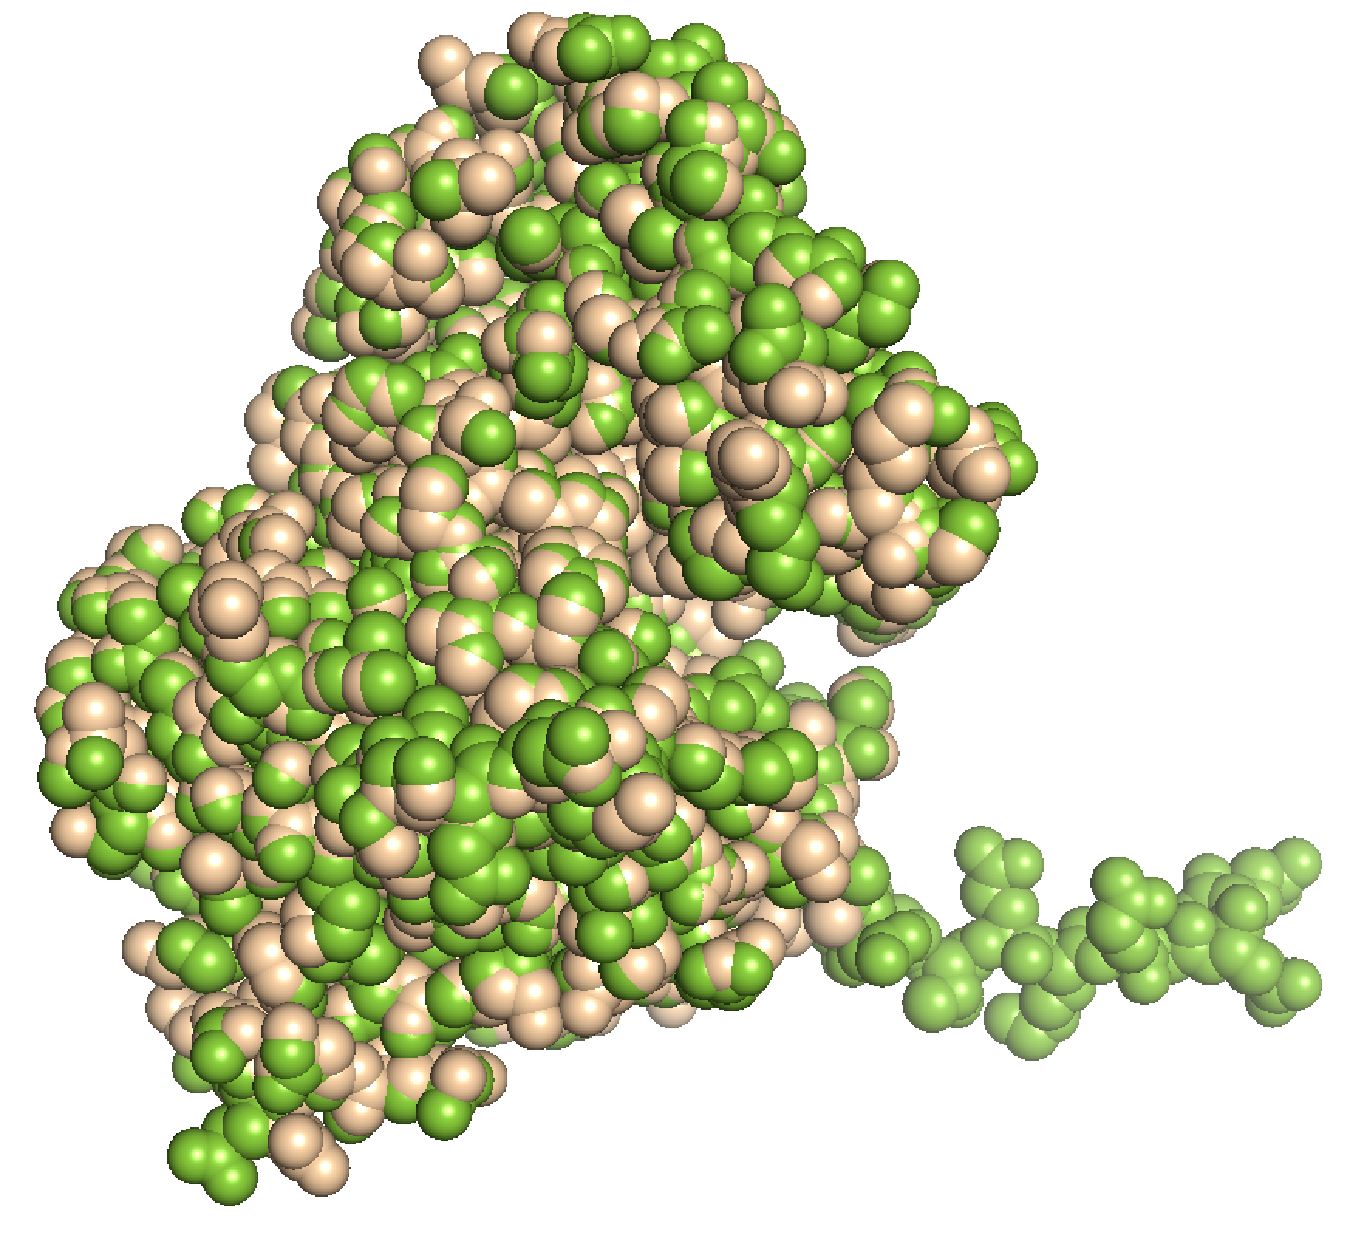
\includegraphics[width=0.3\textwidth]{T0861_Atome2_CBS_TS4.pdf}
	\caption{Пересечение реальной структуры T0861 (жёлтый) и её модели Atome2\textunderscore CBS\textunderscore TS4 (зелёный) при 	$\mathrm{CAD}_\text{score}=0.829$}
	\label{CAD_example}
\end{wrapfigure}

	Обозначим через $G$ множество всех пар элементов последовательности аминокислот (остатков)  $(i, j)$, имеющих ненулевую площадь контакта $T_{(i, j)}$ в реальной структуре. Затем для каждой пары остатков $(i, j)\in G$ вычисляется площадь контакта $M_{(i, j)}$ смоделированной структуры. 
	
	

	Для каждой пары остатков $(i, j) \in G$ определяется разность площадей контакта как абсолютная разница площадей контакта между остатками $i$ и $j$ в реальной $T$ и смоделированной структуре $M$:
	$$\mathrm{CAD}_{(i, j)}=\left|T_{(i, j)}-M_{(i, j)}\right|$$
	
	Для вычислительной стабильности берется ограниченный CAD: $\mathrm{CAD}_{(i, j)}^{\text {bounded}}=\min \left(\mathrm{CAD}_{(i, j)}, T_{(i, j)}\right)$. Таким образом:
	CAD-score для всей структуры определяется как
		\begin{align*}
		\mathrm{CAD}_\text{score}=1-\cfrac{\sum_{(i, j) \in G} \mathrm{CAD}_{(i, j)}^{\text {bounded }}}{\sum_{(i, j) \in G} T_{(i, j)}}
		\end{align*}
	
	\section{Теоретическая часть (?Спектральный анализ?)}
	
	Для обобщения сверточных нейронных сетей на графы необходимо определить сверточные фильтры на графах. Существует два известных подхода: пространственный и спектральный \cite{DBLP:journals/corr/abs-1901-00596, DBLP:journals/corr/abs-1812-08434}. Как показано в \cite{ae482107de73461787258f805cf8f4ed} пространственный подход не имеет общего математического определения трансляции на графах, в то время как  спектральный метод имеет хорошее математическое обоснавание. Поэтому рассматривается спектральная теория графов.
	
	\subsection{Спектральный анализ}
	
	\begin{Def}
		\textit{Графовый Лапласиан} \cite{Chung:1997} -- матрица $\mathbf{L}=\mathbf{I}_{\mathbf{n}}-\mathbf{D}^{-\frac{1}{2}} \mathbf{A} \mathbf{D}^{-\frac{1}{2}}$, где $\mathbf{A}$ -- матрица смежности графа $\mathbf{G}$,  $\mathbf{D}$ -- диагональная матрица степеней вершин, $\mathbf{D}_{i i}=\sum_{j}\left(\mathbf{A}_{i j}\right)$, $\mathbf{I}_{\mathbf{n}}$-- единичная матрица.
	\end{Def}


	
	Матрица $\mathbf{L}$ является вещественной симметричной положительной полуопределенной, поэтому может быть представлена в виде  $\mathbf{L}=\mathbf{U} \mathbf{\Lambda} \mathbf{U}^{T} $, где $\mathbf{U}=\left[\mathbf{u}_{\mathbf{0}}, \mathbf{u}_{\mathbf{1}}, \dots, \mathbf{u}_{\mathbf{n}-\mathbf{1}}\right] \in \mathbb{R}^{n \times n}$ -- это матрица собственных векторов, упорядоченных по собственным значениям, $\boldsymbol{\Lambda} \in \mathbb{R}^{n \times n}$ -- диагональная матрица собственных значений (спектр), $\boldsymbol{\Lambda}_{i i}=\lambda_{i}$. Спектральное разложение Лапласиана позволяет определить преобразование Фурье для графов: собственные векторы соответствуют модам Фурье, а собственные значения -- частотам. 
	
	\begin{Def}
		\textit{Графовое преобразование Фурье}\cite{journals/spm/ShumanNFOV13} для сигнала $\mathbf{x} \in \mathbb{R}^{n}$ задается $\mathscr{F}(\mathbf{x})=\mathbf{U}^{T} \mathbf{x} \equiv \hat{\mathbf{x}} \in \mathbb{R}^{n}$, а обратное графовое пребразование Фурье: $\mathscr{F}^{-1}(\hat{\mathbf{x}})=\mathbf{U} \hat{\mathbf{x}}$, где $\mathbf{x}$ -- вектор признаков всех вершин.
	\end{Def}

	Данное преобразование является ключевым в определении графовой свертки. Оно проецирует входной графовый сигнал на ортонормированное пространство, где базис формируется собственными векторами графового Лапласиана. Элементы преобразованного сигнала $ \hat{\mathbf{x}}$ являются координатами сигнала в новом пространстве, так что входной сигнал может быть представлен как $\mathbf{x}=\sum_{i} \hat{x}_{i} \mathbf{u}_{i}$, что является обратным графовым преобразованием Фурье.
	
	\begin{Theorem}
		\textbf{(Теорема о свертках)}\cite{10.5555/1525499} Преобразование Фурье свертки двух сигналов является покомпонентным произведением их преобразований Фурье, т.е. $$\begin{aligned}\mathscr{F}\left( \mathbf{f} * \mathbf{g}\right) &=\mathscr{F}(\mathbf{f}) \odot \mathscr{F}(\mathbf{g}) \end{aligned}$$
	\end{Theorem}

	Следуя из теоремы, спектральная свертка на графах определяется для сигнала $\mathbf{x}$ и фильтра $\mathbf{g} \in \mathbb{R}^{n}$ как 
	\begin{align}
	\mathbf{x} * \mathbf{g} &=\mathscr{F}^{-1}(\mathscr{F}(\mathbf{x}) \odot \mathscr{F}(\mathbf{g})) =\mathbf{U}\left(\mathbf{U}^{T} \mathbf{x} \odot \mathbf{U}^{T} \mathbf{g}\right) = \mathbf{U g}_{\theta} \mathbf{U}^{T} \mathbf{x},\label{spec_conv}
	\end{align}
	где $\mathbf{g}_{\theta} = \diag\left(\mathbf{U}^{T} \mathbf{g}\right)$ -- спектральные коэффициенты фильтра.
	
	Спектральные методы отличаются выбором фильтра $\mathbf{g}_{\theta}$. Соотношение \ref{spec_conv} вычислительно дорогое, т.к. спектральное разложение требует $O\left(n^{3}\right)$ операций, а перемножение с матрицей собственных векторов $\mathbf{U}$ требует $O\left(n^{2}\right)$ операций. Chebyshev Spectral CNN (ChebNet) \cite{NIPS2016_6081} обходит эти проблемы аппроксимацией $\mathbf{g}_{\theta}$ с помощью полиномов Чебышева $\mathbf{T}_k\mathbf{(x)}$, убирая необходимость считать собственные векторы Лапласиана $\mathbf{L}$.
	
	\begin{Def}
		\textit{Полиномы Чебышева} $\mathbf{T}_k\mathbf{(x)}$ $k$-ого порядкка задаются рекуррентным соотношением  $ \mathbf{T}_{k}(\mathbf{x})=2 \mathbf{x} \cdot \mathbf{T}_{k-1}(\mathbf{x})-\mathbf{T}_{k-2}(\mathbf{x}), \mathbf{T}_{0}(\mathbf{x})=1, \mathbf{T}_{1}(\mathbf{x})=\mathbf{x}$. Образуют ортогональный базис в $L^{2}\left([-1,1], \cfrac{d x} {\sqrt{1-x^{2}}}\right)$
	\end{Def}

	Представляя $\mathbf{g}_{\theta}$ в виде $\mathbf{g}_{\theta}=\sum_{k=0}^{K-1} \theta_{k} \mathbf{T}_{k}\mathbf{(\tilde{\Lambda})}$, где $\mathbf{\tilde{\Lambda}} = 2 \mathbf{\Lambda} / \lambda_{\max }-\mathbf{I}_{n} \in[-1,1]$, $\lambda_{\max }$ -- максимальное собственное число $\mathbf{L}$, а также замечая, что $\left(\mathbf{U} \mathbf{\Lambda} \mathbf{U}^{T}\right)^{k}=\mathbf{U} \mathbf{\Lambda}^{k} \mathbf{U}^{\top}$ (собственные векторы образуют ортонормированный базис $\mathbf{U}^{T}\mathbf{U}=\mathbf{I}$), получаем:
	
	\begin{align}
		\mathbf{U g}_{\theta} \mathbf{U}^{T} \mathbf{x}=\mathbf{U}\left(\sum_{i=0}^{K-1} \theta_{k} \mathbf{T}_{k}(\tilde{\mathbf{\Lambda}})\right) \mathbf{U}^{T} \mathbf{x} = \sum_{k=0}^{K-1} \theta_{k} \mathbf{T}_{k}(\tilde{\mathbf{L}}) \mathbf{x},
		\label{cheb_appr}
	\end{align}
	где $\tilde{\mathbf{L}}=2 \mathbf{L} / \lambda_{\max }-\mathbf{I}_{n}$
	
	Graph Convolutional Network (GCN) \cite{kipf_semi-supervised_2017} используют первое приближение ChebNet. Предполагая $\lambda_{\max} \approx 2$ и $K=1$, соотношение \ref{cheb_appr} упрощается до 
	\begin{align}
	\mathbf{x} * \mathbf{g} \approx \tilde{\theta}_{0} \mathbf{x}+\tilde{\theta}_{1}\left(\mathbf{L}-\mathbf{I}_{N}\right) \mathbf{x}=\tilde{\theta}_{0} \mathbf{x}-\tilde{\theta}_{1} \mathbf{D}^{-\frac{1}{2}} \mathbf{A} \mathbf{D}^{-\frac{1}{2}} \mathbf{x}
	\end{align}
	
	Приняв $\theta = \tilde{\theta}_0  = -\tilde{\theta}_1$, получаем:
	\begin{align}
	\mathbf{x} * \mathbf{g}  \approx \theta\left(\mathbf{I}_{N}+\mathbf{D}^{-\frac{1}{2}} \mathbf{A} \mathbf{D}^{-\frac{1}{2}}\right) \mathbf{x}
	\label{conv}
	\end{align}
	
	Оператор в скобках может может привести к вычислительной нестабильности и взрыву/затуханию градиентов, т.к. собственные значения данного оператора $\in [0,2]$. Для решения проблемы в \cite{kipf_semi-supervised_2017} предлагается \textit{трюк перенормировки}: 
	\begin{align*}
	\mathbf{I}_{N}+\mathbf{D}^{-\frac{1}{2}} \mathbf{A} \mathbf{D}^{-\frac{1}{2}} \rightarrow
	\tilde{\mathbf{D}}^{-\frac{1}{2}} \tilde{\mathbf{A}}\tilde{\mathbf{D}}^{-\frac{1}{2}}, 
	\text{ где }
	\tilde{\mathbf{A}}=\mathbf{A}+\mathbf{I}_{N},~ \tilde{\mathbf{D}}_{i i}=\sum_{j} \tilde{\mathbf{A}}_{i j}
	\end{align*}

	
	\subsection{Сверточный слой}
	
	Дан граф $\mathbf{G}$ и матрица с информацией об узлах $\mathbf{X} \in \mathbb{R}^{n \times c}$ ($n$ -- число узлов и $c$ -- число признаков в каждом узле). Исходя из \ref{conv} и применяя трюк перенормировки, можно определить слой свертки графа таким образом:
	
	$$\mathbf{Z}=\sigma\left(\tilde{\mathbf{D}}^{-1} \tilde{\mathbf{A}}\tilde{\mathbf{D}} \mathbf{X} \mathbf{W}\right),$$
	
	где $\mathbf{W} \in \mathbb{R}^{c \times t}$ – матрица параметров свертки с $t$ фильтрами, $\sigma$ – нелинейная функция активации, а $\mathbf{Z} \in \mathbb{R}^{n \times t}$ -- выходная матрица.
	
		
	
	\section{Данные}
	Берутся с соревнований CASP. Для реальной структуры белка берется еще смоделированная структура. Для них вычисляется CAD-score. Модель на тесте предсказывает CAD-score для смоделированной структуры, не имея возможности напрямую вычислить CAD-score по реальной структуре.
	
\begin{table}[H]
	\begin{minipage}{0.5\linewidth}
		\centering
		\begin{tabular}{l|ll|l}
			\hline Датасет & Таргеты & Модели &  \\
			\hline CASP 7 & 95 & 19591 & \\
			CASP 8 & 122 & 34789 &  { Train/Val } \\
			CASP 9 & 117 & 34946 & \\
			CASP 10 & 103 & 26254 & \\
			\hline 
			CASP 11 & 83 & 16094 & \\
			CASP 12 & 40 & 6924 & Test \\
			\hline
		\end{tabular}
		\caption{Датасеты}
		\label{table:student}
	\end{minipage}\hfill
	\begin{minipage}{0.45\linewidth}
		\centering
		\subfloat[Predicted Atome2\_CBS\_TS4]{\label{fig:edge-a}
			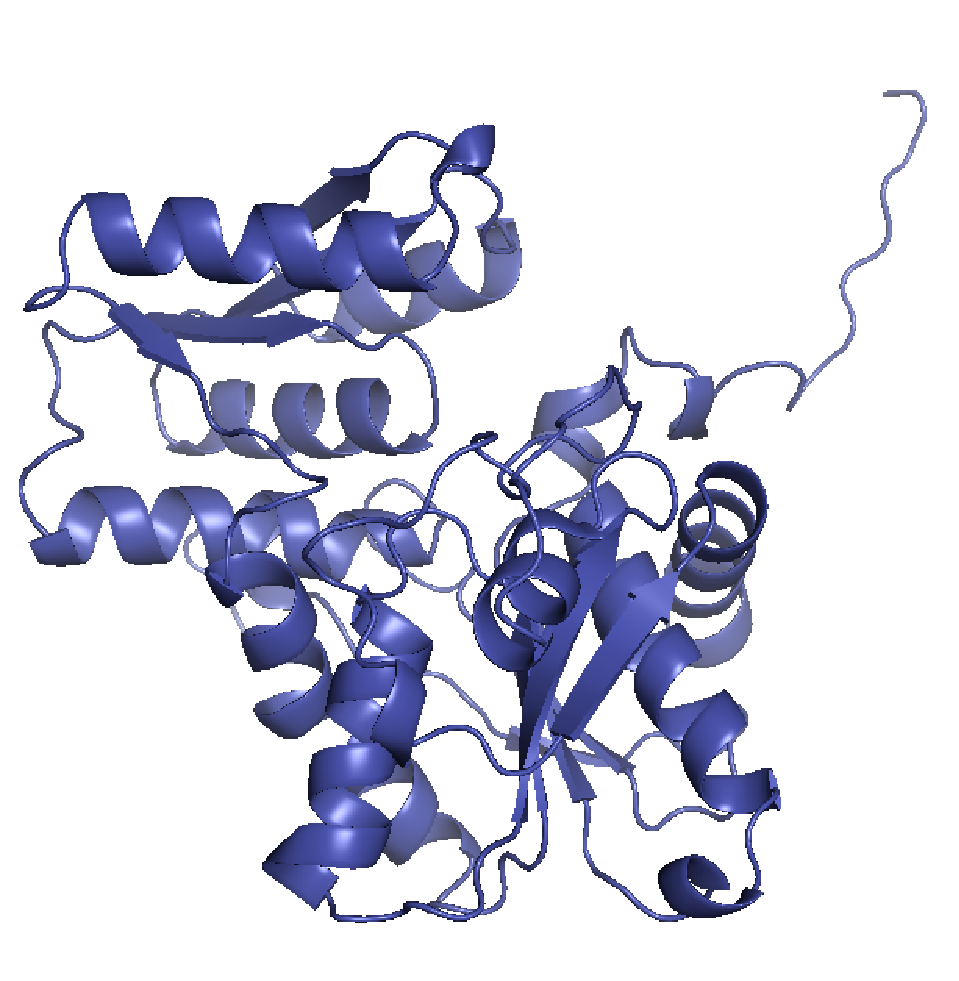
\includegraphics[scale=0.25]{model_T0861.pdf}}
		\subfloat[True]{\label{fig:edge-b}
			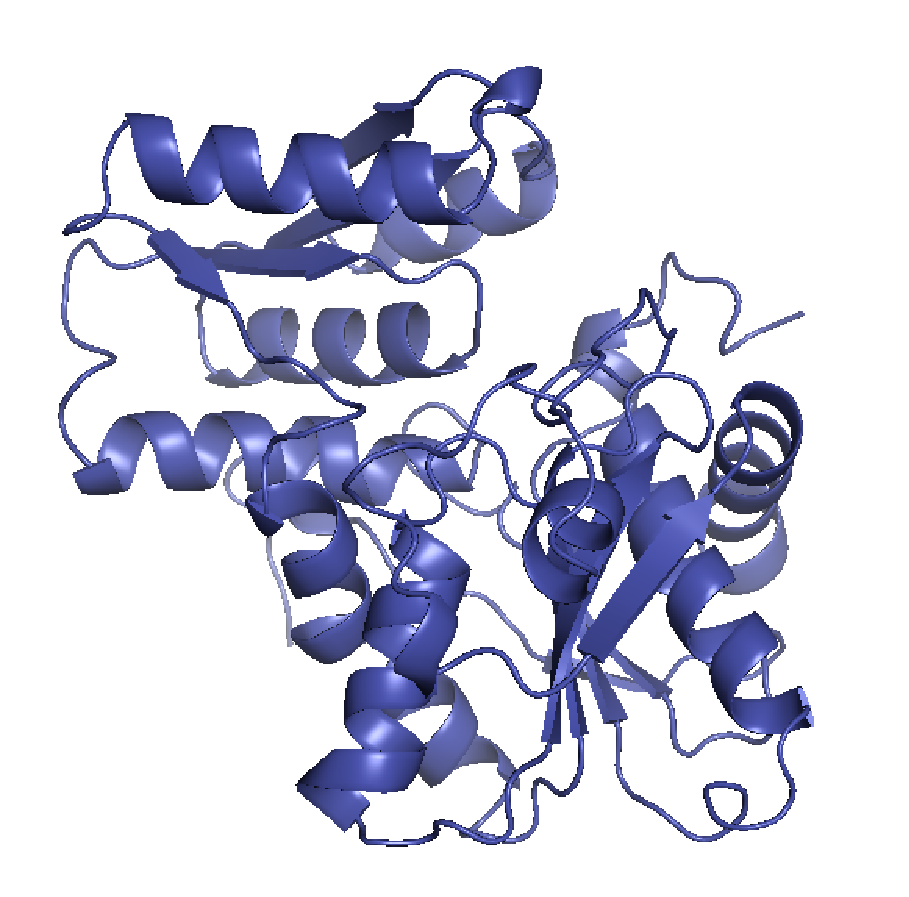
\includegraphics[scale=0.25]{target_T0861.pdf}}
		\captionof{figure}{T0861}
		\label{fig:edge}
	\end{minipage}
\end{table}

	\subsection{Представление белков в виде графов}
	Элементы аминокислотной последовательности рассматриваются как отдельные узлы, чьи связи (ребра) описывают пространственные отношения между ними. 
	
	В общем случае граф $\mathbf{G}$ определяется набором $\mathbf{(V, A)}$, где $\mathbf{V}\in \mathbb{R}^{n \times c}$ определяет вершины или узлы графа. Матрица смежности $\mathbf{A}\in \mathbb{R}^{n \times n}$ определяет соединения между $n$ узлами (ребра), где $\mathbf{A}_{ij}$ – сила связи между узлами $i$ и $j$. Используя это определение графа, белковые структуры можно определить как графы, признаки элементов аминокислотной последовательности которых закодированы в элементах $\mathbf{V}$ узлов, а пространственная близость между элементами закодирована в матрице смежности $\mathbf{A}$.
	

	\subsection{Матрица смежности}
	Т.к. данные о белках не содержат информации о соединениях между атомами, т.е. нет матрицы смежности, построены соединения по следующим правилам:
	\begin{itemize}
		\item не соединяются водород с водородом 
		\item атом не соединяется с водородом, если расстояние между ними $\geq 1.21$ \AA
		\item не соединяются атомы, которые находятся далеко в последовательности (номера остатков отличаются больше, чем на 1)
		\item не соединяются атомы, создающие дисульфидные связи
		\item соединяются атомы, расстояние между которыми $r\in \left(r_{min}, r_{max}\right]$, где $r_{min} = 0.01$\AA, $r_{max} = \left(0.6\cdot(\rho_{atom1}+\rho_{atom2})\right)^2$, $\rho_{atom}$ -- радиус атома (максимально возможное $r_{max} = 5.76$ -- при $\rho_{atom1} = \rho_{atom2} = 2.0$)
	\end{itemize}
	

	\begin{figure}[H]
		\centering
		\begin{minipage}[b]{0.49\textwidth}
			\centering
			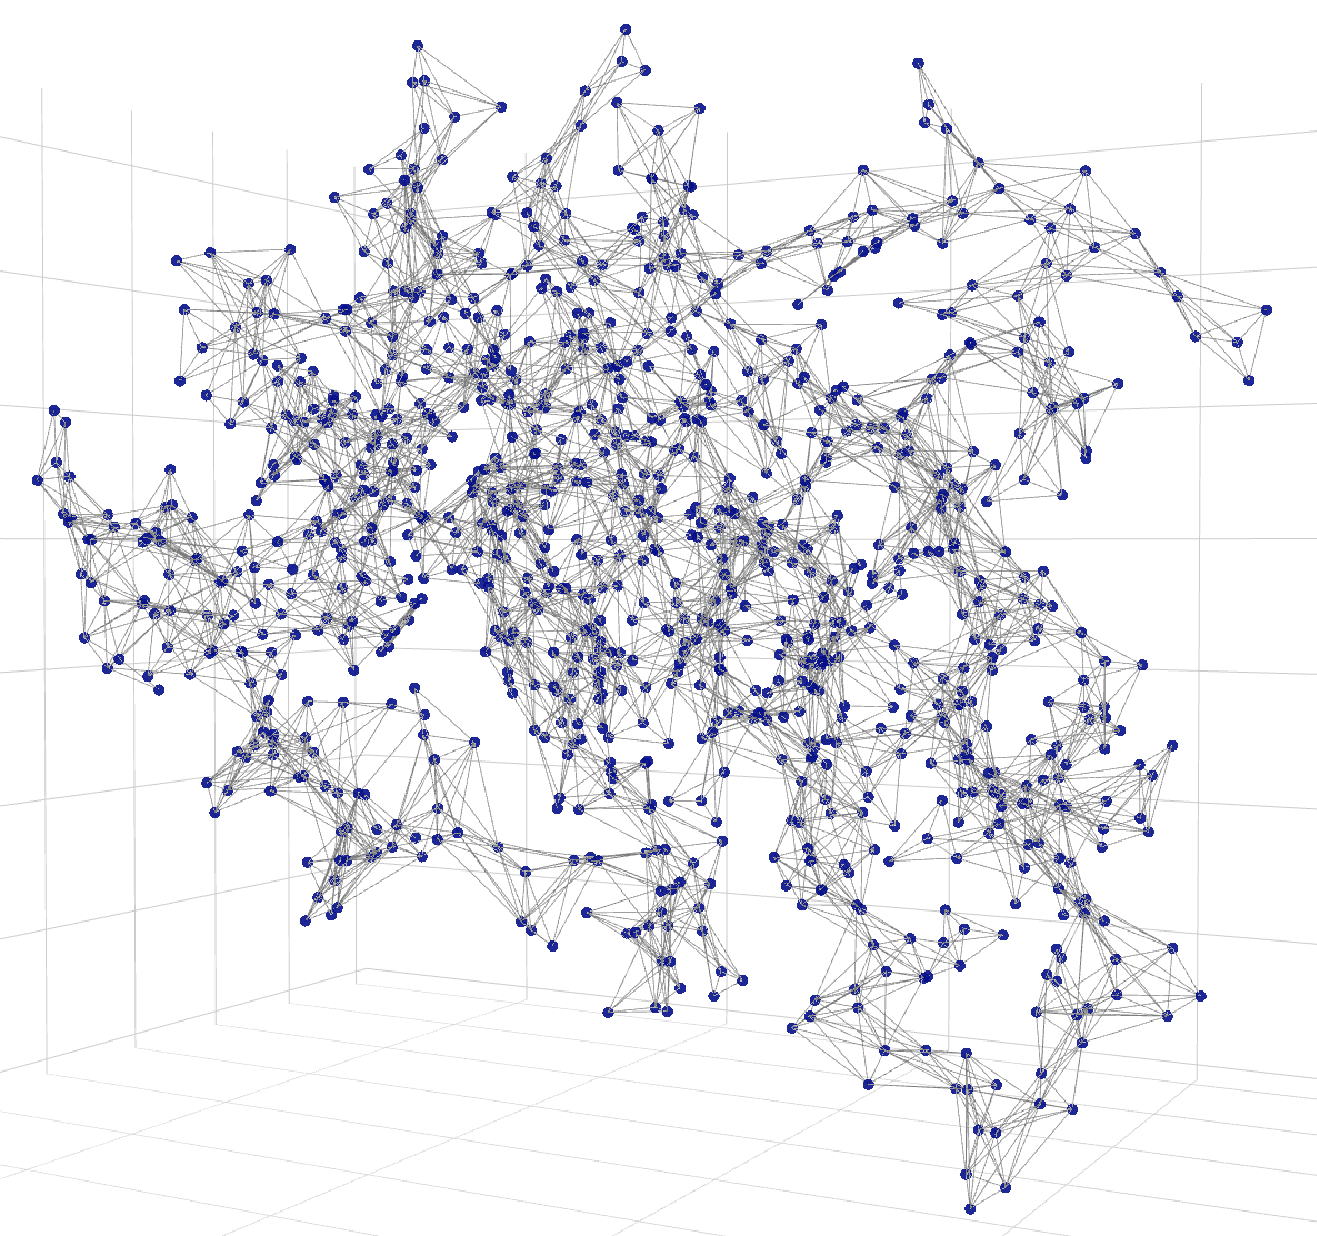
\includegraphics[width=0.9\textwidth]{3d_graph.pdf}
		%	\caption{3D визуализация }
		%	\label{fig:data}
		\end{minipage}
		%\hfill
		\begin{minipage}[b]{0.49\textwidth}
			\centering
			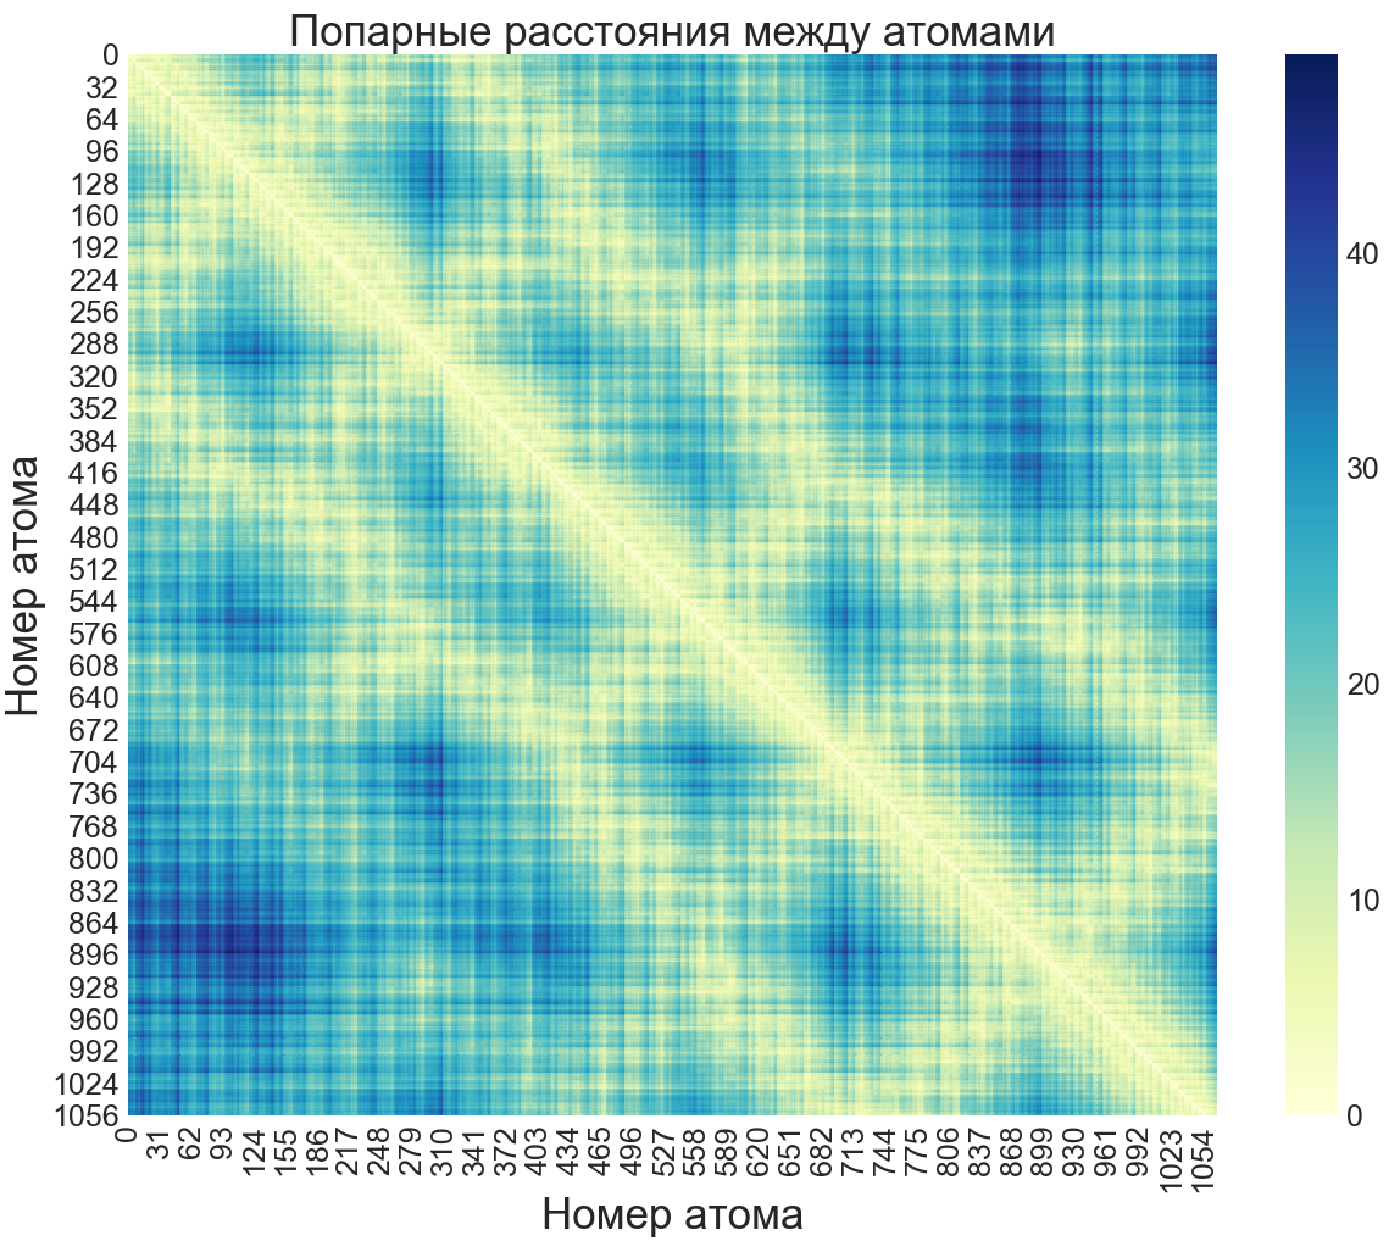
\includegraphics[width=0.9\textwidth]{pairwise.pdf}
		%	\caption{Попарные расстояния между элементами белка}
		%	\label{fig:data}
		\end{minipage}
	\caption{3D представление с помощью координат и полученной матрицы смежности и попарные расстояния между атомами модели модели T0859 BAKER-ROSETTASERVER\_TS2 (CASP12)}
	\label{protein_vis}
	\end{figure}

	По попарным расстояниям между атомами на Рис. \ref{protein_vis} видно, что могут иметь соединения атомы, обозначенные самым светлым желтым, т.к. максимально возможное расстояние между атомами, при котором они могут иметь соединение по представленным правилам составления матрицы смежности -- 5.76 . Т.е. матрица смежности будет сильно разреженной
	
	\section{Вычислительный эксперимент}
		
	
	Варианты архитектур для классификации, основанных на спектральной теории.
	\begin{enumerate}
		%\item Deep Graph Convolutional Neural Network (DGCNN)\cite{Zhang2018AnED}
		\item ChebNet \cite{NIPS2016_6081}
		\item GCN \cite{kipf_semi-supervised_2017}
		\item CayleyNet (???) 
		\item Adaptive Graph Convolution Network (AGCN) (???) 
		\item GRAPH WAVELET NEURAL NETWORK (???) 
	\end{enumerate}
	
	Основа архитектуры берется из существующей модели, где изменяется выходной слой для работы с задачей регрессии.
	
	\subsection{SpectralQA}
	На основе модели GCN
	\begin{figure}[H]
		\centering
		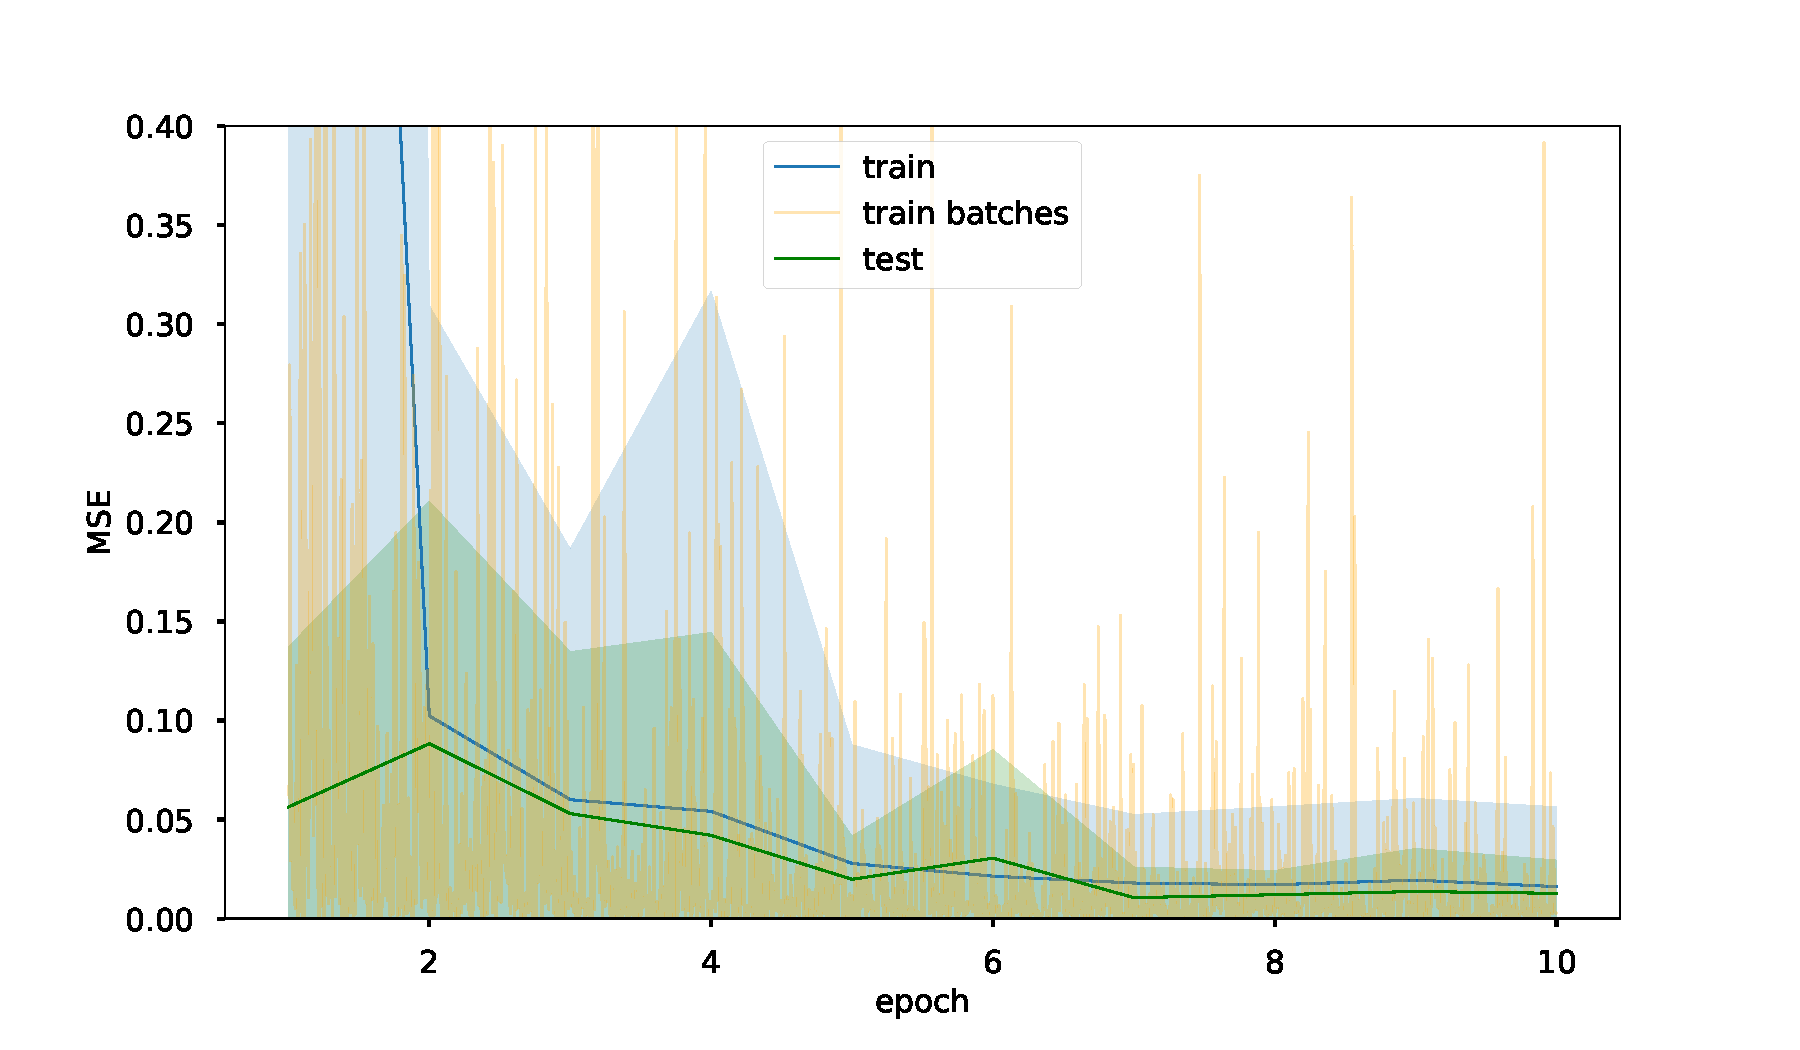
\includegraphics[width=0.9\textwidth]{training.pdf}
		\caption{График MSE ошибки GCN на обучающей и тестовой выборке}
		\label{GCN}
	\end{figure}
	
	\begin{table}[H]
		\centering
		\begin{tabular}{lcr}
			\hline Часть данных & Количество молекул & MSE  \\
			\hline Train & 190 &  \\
			Validation & 31 &   \\
			Test &  &  \\
			\hline
		\end{tabular}
	\end{table}
	
	\section{Результаты и выводы}
	
	Сравнение с существующими методами QA:
	\begin{center}
		\begin{table}[H]
			\centering
			\begin{tabular}{l|l|l|l}
				\hline
				& $\rho$ &  $r$     &    z-score \\ \hline
				ProQ3D     & 0.801  &     11.961     & 1.670       \\
				VoroMQA    & 0.803  &   17.171     & 1.410       \\  
				SBROD      & 0.685  &    23.579     & 1.282       \\
				Ornate     & 0.828  &  0.781    & 1.780       \\
				SpectralQA (МОЯ)&   &      &     
			\end{tabular}
			\caption{Сравнение корреляции Пирсона, Спирмена и z-score существующих современных алгоритмов с моделью SpectralQA на данных CASP12}
			\label{Tab:1}
		\end{table}
	\end{center}
	
	\section{Заключение}
	Впервые для задачи оценки качества прогнозирования структуры белка применены графовые сверточные нейронные сети, в которых свертки определены на основе спектральной теории. В качестве улучшения, можно в основе архитектуры сети пробовать другие существующие улучшения спектральных сверток: CayleyNet, Adaptive Graph Convolution Network (AGCN), GRAPH WAVELET NEURAL NETWORK. Также в будущей работе предлагается учитывать в данных дополнительные свойства атомов и в матрице смежности учитывать не только наличие связи, но и расстояния между атомами при наличии связи.
	
	%\newpage
	\bibliographystyle{plain}
	\nocite{*}
	\bibliography{Severilov2019NIR}
	
\end{document}
